\documentclass[12pt, a4paper]{exam}

% --- 1. FONTS & ENCODING ---
\usepackage[T1]{fontenc}
\usepackage{mathpazo}
\usepackage[scaled=0.95]{helvet}
\usepackage{amsmath, amssymb, gensymb}
\usepackage[version=4]{mhchem}

% --- 2. PAGE GEOMETRY ---
\usepackage{geometry}
\geometry{
    a4paper,
    left=12mm,
    right=12mm,
    top=22mm,
    bottom=20mm,
}

% --- 3. LAYOUT & GRAPHICS PACKAGES ---
\usepackage{graphicx}
\usepackage{multicol}
\usepackage{wrapfig}
\usepackage{tikz}
\usepackage{pgfplots}
\pgfplotsset{compat=1.18}
\usepackage{pdfpages}
\usepackage{background}
\usepackage{enumitem}
\usepackage{booktabs}
\usepackage{array}

% --- 4. SECTION BOX ---
\usepackage{tcolorbox}
\tcbuselibrary{skins}

\newtcolorbox{sectionbox}{
    enhanced,
    colback=black!8!white,
    colframe=black!75!white,
    boxrule=1.2pt,
    arc=3pt,
    width=\linewidth,
    halign=center,
    valign=center,
    fontupper=\sffamily\bfseries\large,
    top=4pt,
    bottom=4pt,
}

\newcommand{\boxsection}[1]{%
    \par\vspace{0.6em}\noindent
    \begin{sectionbox}
        #1
    \end{sectionbox}
    \vspace{0.5em}
}

% --- 5. SUBSECTION STYLING ---
\usepackage{titlesec}
\titleformat{\subsection}[block]
  {\normalfont\sffamily\bfseries\normalsize\underline}
  {}
  {0pt}
  {}
\titlespacing{\subsection}{0pt}{0.7em}{0.3em}

% --- 6. WATERMARK ---
\backgroundsetup{
  scale=14,
  color=gray,
  opacity=0.12,
  angle=45,
  position=current page.center,
  contents={TRINITY}
}

% --- 7. EXAM CLASS SETTINGS ---
\pointsdroppedatright
\pointsinrightmargin

% --- 8. COLUMN SEPARATOR ---
\setlength{\columnsep}{1cm}

% --- 9. IMAGE PATH ---
\graphicspath{{../}{images/}}

\newcommand{\qimg}[2][0.95]{%
    \par\vspace{0.4em}%
    \includegraphics[width=#1\linewidth]{#2}%
    \par\vspace{0.2em}%
}

% -------------------------------------------------------

\begin{document}

\begin{center}
    {\sffamily\bfseries\Large TRINITY CENTRE FOR LEARNING}\\[2pt]
    {\sffamily\large CLASS XI -- PHYSICS}\\[2pt]
    {\sffamily\normalsize Surface Tension $|$ Angle of Contact \& Capillary Rise}
\end{center}
\vspace{0.3em}
\noindent\rule{\linewidth}{0.8pt}
\vspace{0.3em}

% ============================================================
\boxsection{NOTES}
% ============================================================

\begin{multicols}{2}

\subsection*{Angle of Contact}

The \textit{angle of contact} $\theta$ is the angle between the tangent to the liquid surface at the point of contact and the solid surface, measured \emph{inside} the liquid.

\begin{itemize}[leftmargin=*, itemsep=2pt]
    \item \textbf{Acute} ($\theta < 90^\circ$): liquid \textit{wets} the solid (e.g.\ water on glass, $\theta \approx 0^\circ$--$8^\circ$). Meniscus is \textbf{concave}.
    \item \textbf{Obtuse} ($\theta > 90^\circ$): liquid \textit{does not wet} the solid (e.g.\ mercury on glass, $\theta \approx 135^\circ$). Meniscus is \textbf{convex}.
    \item \textbf{Right angle} ($\theta = 90^\circ$): flat meniscus; no net wetting tendency.
\end{itemize}

The angle of contact depends on the nature of the liquid-solid pair and is independent of the tilt of the surface.

\subsection*{Cohesion, Adhesion \& Meniscus Shape}

\begin{itemize}[leftmargin=*, itemsep=2pt]
    \item \textbf{Cohesion}: attraction between like molecules (liquid--liquid).
    \item \textbf{Adhesion}: attraction between unlike molecules (liquid--solid).
    \item If adhesion $>$ cohesion $\Rightarrow$ concave meniscus (water in glass).
    \item If cohesion $>$ adhesion $\Rightarrow$ convex meniscus (mercury in glass).
\end{itemize}

\subsection*{Capillary Rise / Depression}

A liquid rises (or falls) in a narrow tube of radius $r$ due to surface tension $T$. Equating the upward pull of surface tension to the weight of the liquid column:

\[
    h = \frac{2T\cos\theta}{\rho g r}
\]

where:
\begin{itemize}[leftmargin=*, itemsep=2pt]
    \item $T$ = surface tension of the liquid (N\,m$^{-1}$)
    \item $\theta$ = angle of contact
    \item $\rho$ = density of liquid (kg\,m$^{-3}$)
    \item $g$ = acceleration due to gravity (m\,s$^{-2}$)
    \item $r$ = radius of the capillary (m)
\end{itemize}

\textbf{Key deductions from the formula:}
\begin{enumerate}[leftmargin=*, itemsep=2pt]
    \item $h \propto \dfrac{1}{r}$: narrower tube $\Rightarrow$ greater rise.
    \item $h \propto T$: higher surface tension $\Rightarrow$ greater rise.
    \item $h \propto \cos\theta$: smaller $\theta$ $\Rightarrow$ greater rise.
    \item For $\theta > 90^\circ$ (e.g.\ mercury), $\cos\theta < 0 \Rightarrow h < 0$: \textbf{capillary depression}.
\end{enumerate}

\subsection*{Effect of Temperature}

Surface tension decreases with increasing temperature. From $h = 2T\cos\theta/\rho g r$, a rise in temperature lowers $T$, so the capillary height $h$ decreases.

\subsection*{Jurin's Law}

For a given liquid--solid system ($T$, $\theta$, $\rho$ fixed):
\[
    h \cdot r = \text{constant} = \frac{2T\cos\theta}{\rho g}
\]
Doubling the radius halves the capillary rise.

\end{multicols}

\vspace{0.4em}
\noindent\rule{\linewidth}{0.4pt}
\vspace{0.2em}

% Capillary diagram
\begin{center}
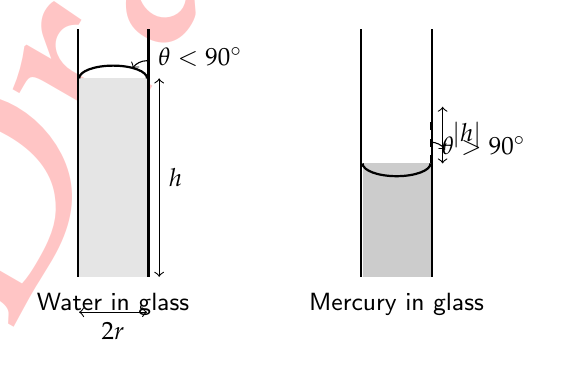
\begin{tikzpicture}[scale=0.9]
  % --- Capillary rise (water, concave meniscus) ---
  \begin{scope}[xshift=0cm]
    % tube walls
    \draw[thick] (-0.5, 0) -- (-0.5, 3.5);
    \draw[thick] ( 0.5, 0) -- ( 0.5, 3.5);
    % liquid fill
    \fill[gray!20] (-0.48, 0) rectangle (0.48, 2.8);
    % concave meniscus
    \draw[thick] (-0.48, 2.8) arc[start angle=180, end angle=0, x radius=0.48, y radius=0.18];
    % angle of contact annotation
    \draw[dashed] (0.48, 2.8) -- (0.48, 3.3);
    \draw[->, thin] (0.48, 3.05) arc[start angle=90, end angle=145, radius=0.25];
    \node[right, font=\small] at (0.5, 3.1) {$\theta < 90^\circ$};
    % height arrow
    \draw[<->] (0.65, 0) -- (0.65, 2.8) node[midway, right, font=\small]{$h$};
    % label
    \node[below, font=\sffamily\small] at (0, -0.1) {Water in glass};
  \end{scope}

  % --- Capillary depression (mercury, convex meniscus) ---
  \begin{scope}[xshift=4cm]
    % tube walls
    \draw[thick] (-0.5, 0) -- (-0.5, 3.5);
    \draw[thick] ( 0.5, 0) -- ( 0.5, 3.5);
    % liquid fill (lower level inside)
    \fill[gray!40] (-0.48, 0) rectangle (0.48, 1.6);
    % convex meniscus
    \draw[thick] (-0.48, 1.6) arc[start angle=180, end angle=0, x radius=0.48, y radius=-0.18];
    % angle of contact annotation
    \draw[dashed] (0.48, 1.6) -- (0.48, 2.2);
    \draw[->, thin] (0.48, 1.9) arc[start angle=90, end angle=35, radius=0.25];
    \node[right, font=\small] at (0.5, 1.85) {$\theta > 90^\circ$};
    % depression arrow
    \draw[<->] (0.65, 1.6) -- (0.65, 2.4) node[midway, right, font=\small]{$|h|$};
    % label
    \node[below, font=\sffamily\small] at (0, -0.1) {Mercury in glass};
  \end{scope}

  % radius label for left tube
  \draw[<->] (-0.48, -0.5) -- (0.48, -0.5) node[midway, below, font=\small]{$2r$};
\end{tikzpicture}
\end{center}

\vspace{0.3em}
\noindent\rule{\linewidth}{0.4pt}

% ============================================================
\boxsection{WORKSHEET}
% ============================================================

\begin{multicols}{2}

\subsection*{Short Answer}

\begin{questions}

\question Define angle of contact. State its value for a perfectly wetting liquid. \dotfill \hfill\makebox[1.5cm]{\dotfill}
\vspace{2em}

\question Explain why the meniscus of water in a glass capillary is concave while that of mercury is convex.
\vspace{3em}

\question State two factors on which the angle of contact depends. Does it depend on the inclination of the capillary? Justify.
\vspace{3em}

\question Write the formula for capillary rise and define each symbol. \hfill\makebox[1.5cm]{\dotfill}
\vspace{2em}

\question A capillary tube is held vertically in a liquid that wets glass. Describe and explain what happens when the tube is progressively narrowed.
\vspace{3em}

\subsection*{Numerical}

\question A capillary tube of radius $0.4 \times 10^{-3}$ m is dipped vertically in water. Given $T = 0.072$ N\,m$^{-1}$, $\rho = 1000$ kg\,m$^{-3}$, $g = 9.8$ m\,s$^{-2}$, and $\theta = 0^\circ$, calculate the height of water in the tube. \hfill[3]

\vspace{4em}

\question Water rises to a height of 9 cm in a capillary of radius $r$. What will be the height of rise if the radius is reduced to $r/3$? \hfill[2]

\vspace{3em}

\question The surface tension of mercury is $0.465$ N\,m$^{-1}$ and its angle of contact with glass is $135^\circ$. Find the capillary depression in a tube of radius $0.5$ mm. ($\rho_{\text{Hg}} = 13600$ kg\,m$^{-3}$, $g = 9.8$ m\,s$^{-2}$.) \hfill[3]

\vspace{4em}

\question A liquid rises 4 cm in a capillary at $20^\circ$C. If the surface tension of the liquid decreases by 20\% when heated to $60^\circ$C (all other quantities unchanged), find the new height of rise. \hfill[2]

\vspace{3em}

\subsection*{Application / Reasoning}

\question Why does a fine-tipped pen hold ink but a wide nib requires pressure to write? Use Jurin's Law in your answer.
\vspace{3em}

\question Explain how the waterproofing of fabric relies on angle of contact. What change is introduced in the surface to achieve this?
\vspace{3em}

\question \textit{Assertion:} Capillary rise is independent of the shape of the capillary.\\
\textit{Reason:} At equilibrium, only the radius at the meniscus determines the rise.\\
State whether the assertion and reason are correct and whether the reason is the correct explanation of the assertion. \hfill[2]
\vspace{3em}

\end{questions}

\end{multicols}

% ============================================================
\boxsection{PREVIOUS YEAR QUESTIONS}
% ============================================================

\begin{multicols}{2}
\begin{questions}

\question Define surface tension. A liquid rises to a height of 7 cm in a capillary tube of radius $0.1$ mm. Another liquid of density half the first and surface tension two-thirds that of the first rises to a height of \rule{1.5cm}{0.15mm} in a capillary of radius $0.05$ mm (angle of contact $= 0^\circ$ for both). \hfill\textbf{[ICSE 2019]}

\vspace{3em}

\question The angle of contact between glass and mercury is $135^\circ$. A narrow tube of radius $0.02$ cm is partially immersed in mercury. Find the depression of mercury in the tube. ($T_{\text{Hg}} = 0.5$ N\,m$^{-1}$; $\rho = 13600$ kg\,m$^{-3}$.) \hfill\textbf{[ICSE 2018]}

\vspace{4em}

\question State Jurin's Law. Two capillary tubes of radii $r$ and $4r$ are dipped in the same liquid. Compare the heights to which the liquid rises. \hfill\textbf{[ICSE 2017]}

\vspace{3em}

\question What is the effect of temperature on (i) surface tension and (ii) capillary rise? Give reasons. \hfill\textbf{[ICSE 2016]}

\vspace{3em}

\question A capillary tube of uniform bore is dipped vertically in water which rises to a height of $h$. If a liquid of density $0.8 \rho$ and surface tension $0.6T$ (angle of contact $0^\circ$) is used instead, find the new height of rise in terms of $h$. \hfill\textbf{[ISC 2022]}

\vspace{3em}

\question Choose the correct option.\\
The meniscus of mercury in a glass capillary is convex because:

\vspace{0.3em}
\begin{choices}
\choice Adhesive force between mercury and glass is greater than cohesive force within mercury
\choice Cohesive force within mercury is greater than adhesive force between mercury and glass
\choice Surface tension of mercury is very high
\choice Mercury has high density \hfill\textbf{[NEET 2021]}
\end{choices}

\vspace{0.5em}

\question Water rises in a capillary tube to a height of $h$. If the same capillary tube is inclined at $60^\circ$ to the vertical, the length of water column in the tube is:

\vspace{0.3em}
\begin{oneparchoices}
\choice $h/2$
\choice $h$
\choice $2h$
\choice $h\sqrt{3}$ \hfill\textbf{[JEE 2020]}
\end{oneparchoices}

\vspace{0.5em}

\question If a capillary tube is immersed in water and then taken out and its lower end is sealed, what happens to the water in the tube? Explain with reference to surface tension and pressure. \hfill\textbf{[ICSE 2015]}

\vspace{3em}

\end{questions}
\end{multicols}

\end{document}
